%        File: RegressionToTheMean.tex
%     Created: Thu Jan 29 11:00 AM 2015 E
% Last Change: Thu Jan 29 11:00 AM 2015 E
%
\documentclass[12pt]{article}
\title{Conditional Probability\\ \large Monty Hall problem}
\author{Econ 103}
\usepackage{graphicx}
\usepackage{amsmath}

\begin{document}
\maketitle

\section*{Question}

Suppose you're on a game show, and you're given the choice of three doors: Behind one door is a car; behind the others, goats. You pick a door, say No. 1, and the host, who knows what's behind the doors, opens another door, say No. 2, which has a goat. He then says to you, "Do you want to pick door No. 3?" Is it to your advantage to switch your choice? 


\begin{center}
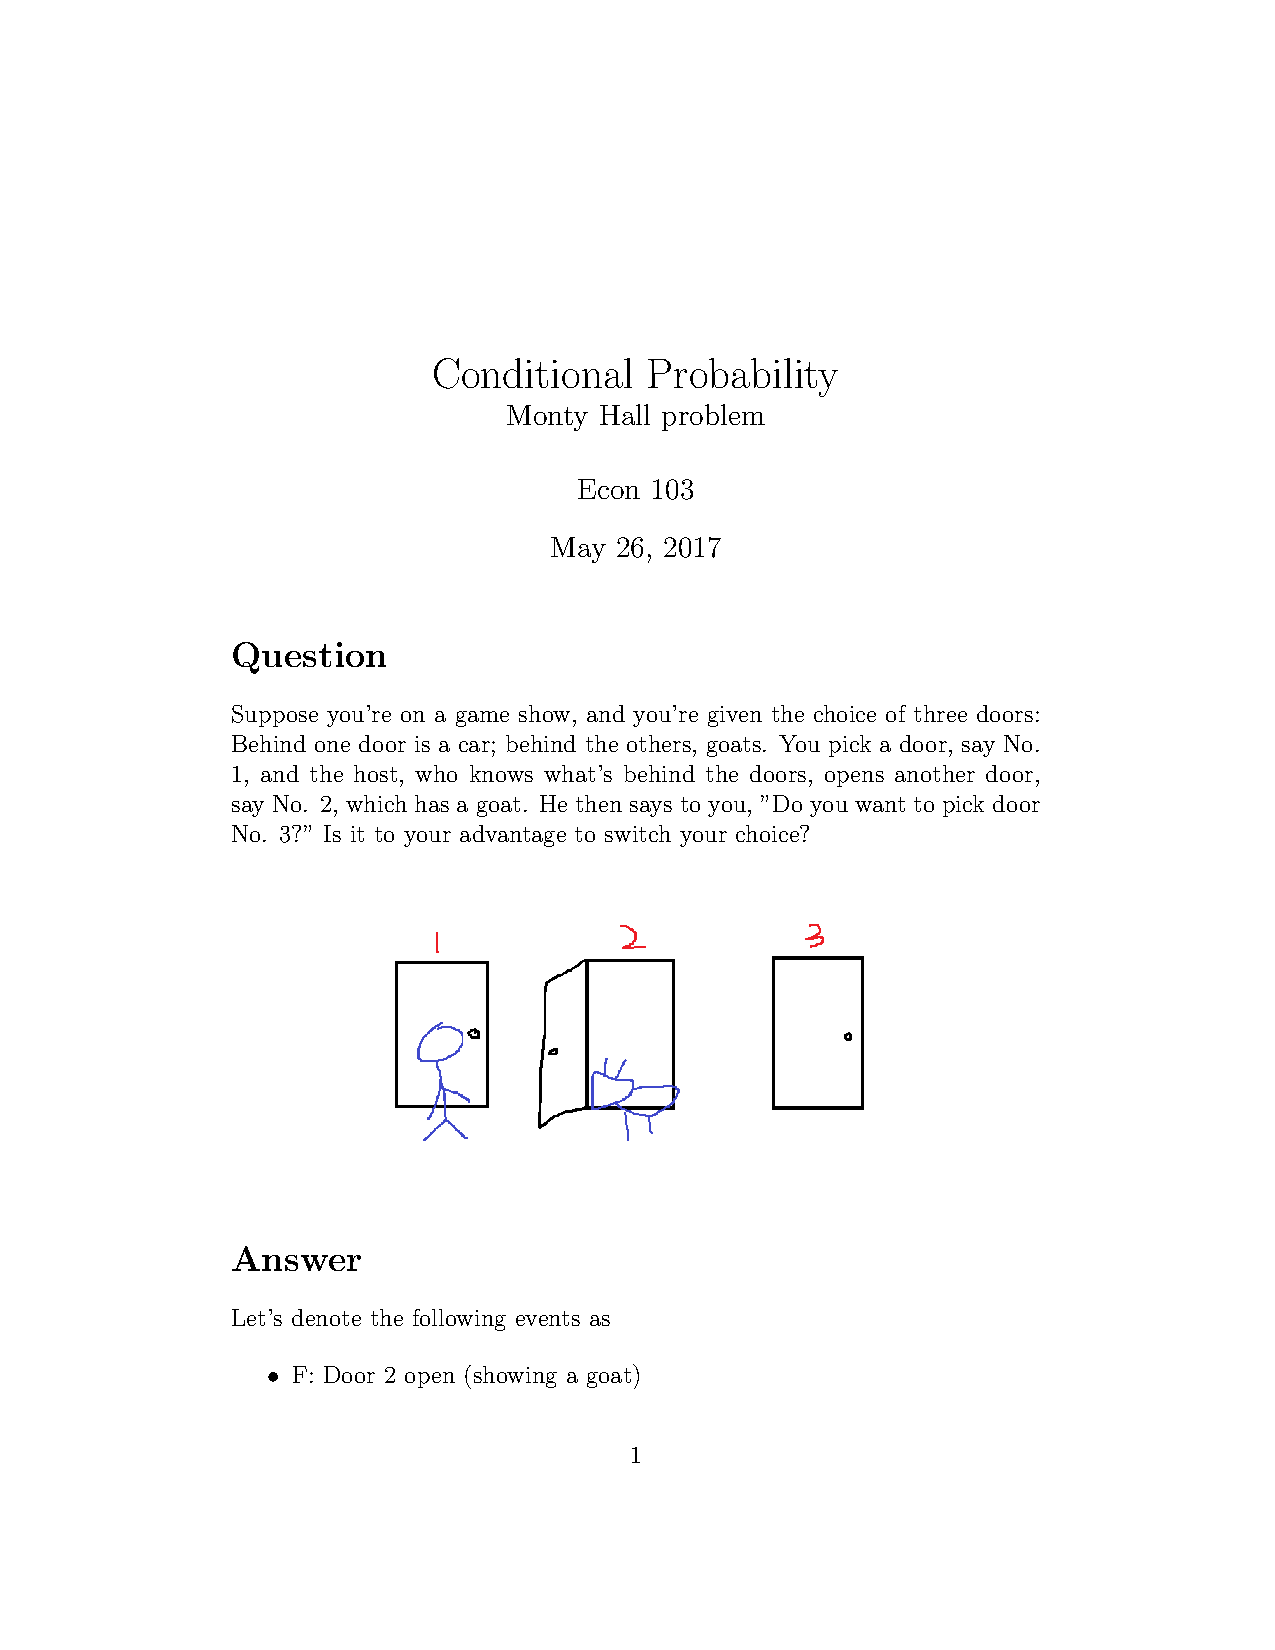
\includegraphics[scale = 0.45]{MontyHall}
\end{center}

\section*{Answer}

Let's denote the following events as

\begin{itemize}
\item F: Door 2 open (showing a goat)
\item A: Car behind 1
\item B: Car behind 2
\item C: Car behind 3
\end{itemize}

We know that $P(A) = P(B) = P(C) = \frac{1}{3}$.
The probability we need to compute is $P(A|F)$. Using the definition of  conditional probability, 

\[
P(A|F) = \frac{P(A \cap F)}{P(F)}
\] 

Let's first start with $P(A \cap F)$. 

\[
P(A\cap F) = P(F|A)P(A) = \frac{1}{2} \times \frac{1}{3} = \frac{1}{6}.
\]

Conditional probability $P(F|A)$ is $\frac{1}{2}$ since the host can choose whether to open the door 2 or 3 when the door 1 is chosen already.\\
Let's move on to compute $P(F)$. We can see that the events $A, B, C$ are mutually exclusive and collectively exhaustive. We can use the law of total probability as follows:

\begin{align*}
P(F) &= P(F|A)P(A) + P(F|B)P(B) + P(F|C)P(C)\\
& = \frac{1}{2} \times \frac{1}{3} + 0 \times \frac{1}{3} + 1 \times \frac{1}{3} = \frac{1}{2}
\end{align*}

Notice that $P(F|C) = 1$. If the car is behind the door 3, then the host has no option but to open the door 2 to show the goat. Therefore, we know that

\[
P(A|F) = \frac{\frac{1}{6}}{\frac{1}{2}} = \frac{1}{3}
\]

Using the complement rule, we know $P(A^C|F) = 1-P(A|F) = \frac{2}{3}$. Therefore, it is better to pick the door 3! (Also, note that $P(A|F) = P(A)$. This means that $A$ and $F$ are independent events.)



\end{document}
